\chapter{Dedução - Argumento}

Um dos principais objetivos do estudo da Lógica é o de estabelecer métodos e técnicas que permitam distinguir os raciocínios corretos dos incorretos.
Em um tipo especial de raciocínio denominado RACIOCÍNIO DEDUTIVO ou DEDUÇÃO, faz-se necessário o exame da relação existente entre uma determinada conclusão e as razões que lhes serviram de "apoio".

O estudo do ARGUMENTO é, assim, um dos pontos centrais do estudo da Lógica.

Chamamos de ARGUMENTO a uma sequência finita de enunciados, onde os primeiros (PREMISSAS) "apoiam" ou "servem de evidência" para o último enunciado (CONCLUSÃO).

% Por questões de simplicidade, usei uma imagem para representar o diagrama a seguir. O código dele está abaixo, porém ele foi gerado em um documento limpo (gerando aqui o resultado é diferente)
\begin{comment}
    \begin{forest}
        for tree={
        grow=west,
        s sep=.1em,
        l sep=3em,
        sn edges
        }
        [Argumento
        [Premissas
        [$P_1$, tier=prem]
        [$\vdots$, tier=prem, no edge]
        [$P_{n-1}$, tier=prem]
        ]
        [Conclusão
        [$P_n$, tier=prem, edge={<-}]
        ]
        ]
        \draw (-8.1,-0.7) -- (-7,-0.7);
        \end{forest}
\end{comment}

\begin{figure}[H]
	\begin{center}
	    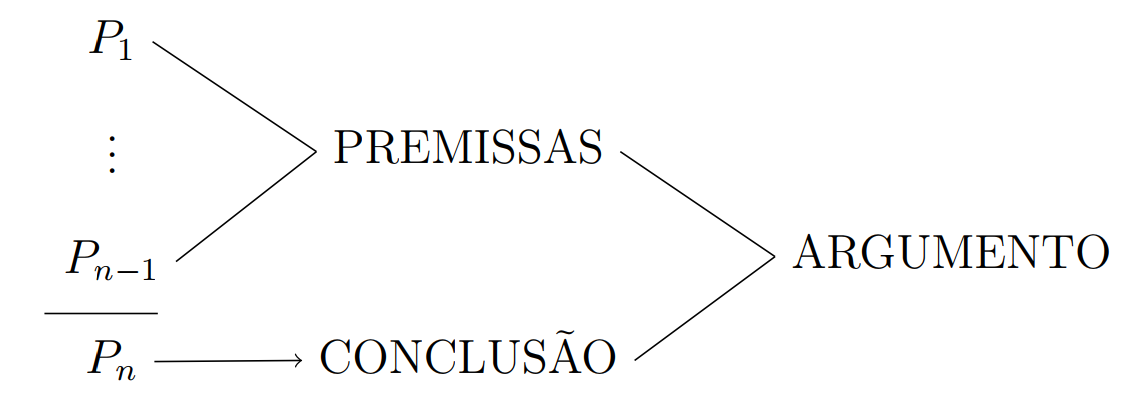
\includegraphics[scale=0.3]{diagramaCapitulo5Grande.png}
	\end{center}
\end{figure}

Diz-se que um argumento é DEDUTIVAMENTE VÁLIDO quando é impossível que a conclusão seja falsa partindo-se de premissas verdadeiras, ou seja, quando a conclusão é consequência lógica das premissas.
Caso contrário, o argumento é dito DEDUTIVAMENTE INVÁLIDO.

Evidentemente será do nosso interesse apenas o estudo dos argumentos dedutivamente válidos.

Vejamos os exemplos:

\begin{align*}
    (ii) & \text{ Se Carla chegar, ganhará a aposta.}\\
         & \text{ Se Carla ganhar a aposta, viajará.}\\
    \text{Logo,}\\
         & \text{ Se Carla chegar, viajará.}
\end{align*}

É importante ressaltar o fato da atenção necessária ao encaminhamento de um raciocínio, a fim de que não se caia em "armadilhas", que nos levam a acreditar que uma forma errada de raciocinar é correta.
Tais formas de argumento ou raciocínio são chamadas de FALÁCIAS.
Por exemplo:

\begin{quote}
    Os estudantes que estudam obtém nota dez. Logo, o melhor que o professor tem a fazer é dar nota dez aos seus alunos.
\end{quote}
